\documentclass{article}

\usepackage[T1]{fontenc}    %Schriftart des Dokumentes
\usepackage[british]{babel} %Dokumentensprache, hier Deutsch
\usepackage{amsmath, amssymb, stmaryrd} %mathematische Schriftzeichen
\usepackage{graphicx} %Einfügen von Grafiken
\usepackage{wrapfig}
\usepackage{bm}

\setlength{\parindent}{0pt} %Einrückung von Absätzen auf null gesetzt
\setlength{\parskip}{10pt} %Abstand zischen Absätzen auf 10pt gesetzt

\title{Experiment 41: Temperature measurement}
\author{Matthias Kuntz}
\date{13.09.2023}

\begin{document}

\maketitle

%-------------------------EINLEITUNG-------------------------
\section{Introduction}

In this experiment we will take measurements in different temperature ranges and with different thermometers to see how well they compete in certain situations compared to each other. Firstly, we will be using a gas thermometer, a platinum resistance thermometer, and a infrared thermometer to record temperatures ranging from 0$^{\circ}$C up to 100$^{\circ}$C. Then, using only the gas and platinum resistance thermometers we will go below zero to measure the temperatures of dry ice as well as liquid nitrogen. Finally, we will use a thermocouple to record the temperature distribution of a Bunsen burner flame.

\subsection{Basics}

In this section we will discuss the different kinds of thermometers used and how they work.

\textbf{Gas thermometer:}

Firstly, the gas thermometer operates on the principle of the ideal gas equation:

\begin{equation}
    pV = NkT
\end{equation}

Where $p$ is pressure, $V$ volume, $N$ the number of particles, $k$ the Boltzmann constant, and $T$ the temperature. 

Assuming the gas used in the thermometer is mostly ideal, we can derive the relation that within the closed container of the thermometer, the pressure inside is only dependant on the temperature. Often times gases like Helium or Hydrogen  are used, since their behaviour matches the one of an ideal gas the most over a wide range of temperatures. Figure 1 of the measurement protocol shows a simple sketch of the setup of a gas thermometer. The glass balloon is filled with the gas and the capillary connects to a manometer to record the pressure.

When working with gas thermometers, systematic errors need to be taken into account. First, we need to mention the fact that the glass ball expands when heated up. But since the gas inside expands quicker because of it's much larger expansion coefficient compared to the glass ball, this error can be safely neglected. Second, when exposing the glass ball to temperature shifts, the air between the ball and the capillary mostly stays unaffected at room temperature, creating a sort of "harmful volume" when the glass container starts expanding or compressing. Finally, we need to consider the fact that no gas is ideal and that at certain temperatures effects like the liquefaction of the gas may occur. But in our experiments conditions for these cases are not met.

\textbf{The platinum resistance thermometer:}

A platinum resistance thermometer works on the principle that the electrical resistance depends on the temperature. In this experiment, a constant current of 1 mA is applied to the resistor and the voltage falloff across the resistor is measured by a voltmeter. The temperature dependence can be sufficiently determined by a second degree polynomial:

\begin{equation}
    \begin{split}
        R(T) &= R_0 (1+AT+BT^2) \\ \\
        & \text{where} \\ \\
        A &= 3,9083 \cdot 10^{-3} [^{\circ}\text{C}^{-1}] \\
        B&= -5,775 \cdot 10^{-7} [^{\circ}\text{C}^{-2}]
    \end{split}
\end{equation}

Which includes the resistance $R(T)$, temperature $T$, the constants $A$ and $B$, as well as the nominal resistance at 0$^{\circ}$C $R_0$, which is given as 100 $\Omega$ for a Pt100. 

Having calculated the resistance using Ohm's law, we can determine the temperatures according to:

\begin{equation}
    \begin{split}
        T(R) &= \frac{-R_0A + \sqrt{RR_0^2A^2 - 4R_0B(R_0-R)}}{2R_0B} \\
        \Delta T &= 0,30 ^{\circ}\text{C} + 0,005 \cdot |T|
    \end{split}
\end{equation}

\newpage

When taking measurements of the voltage, we need to consider the drop over the cables, which also have an electrical resistance. To avoid this problem, a special four wire circuit is used, which is shown in figure 1.

\begin{figure} [!ht]
    \centering
    \includegraphics[width=12cm]{graphics/sketch2.jpg}
    \caption{two (left) and four (right) wire circuits for the Pt100 thermometer}
\end{figure}

\textbf{The pyrometer:}

The pyrometer measures the thermal radiation emitted by any body with a temperature greater than 0K. To function, it assumes every measured object to be a perfect black radiator, which is a body that absorbs all electromagnetic radiation, meaning the emitted intensity is only dependent on the temperature. The intensity distribution of a black radiator is described by Planck's radiation law:

\begin{equation}
    M_{\lambda} (\lambda, T) \ dA \ d \lambda = \frac{2 \pi h c^2}{\lambda^5} \frac{1}{e^{\left( \frac{hc}{\lambda k T} \right)}-1} \ dA \ d \lambda 
\end{equation}

\textbf{The thermocouple:}

The thermocouple operates based on the Seebeck effect, which states that if two different metals are brought in contact with each other, an electric voltage $U_{th}$ builds up at the contact point, whose amount depends on the type of metals used as well as the temperature at the contact point $T_1$ and at both ends of the metals $T_2$:

\begin{equation}
    U_{th} = K(T_1 - T_2)
\end{equation}

Here, $K$ is a constant which depends on the type of both metals. 

When working with thermocouples it is important to keep in mind that only relative temperatures can be measured. To determine one of the temperatures absolutely demands knowing the other one already. For our experiment, a simple thermocouple as described above using the room temperature as $T_2$ is sufficient.

\subsection{Experiment Setup}

A sketch of the setup can be found on the next page in the measurement protocol. 

For this experiment, we will start by comparing the two and four wire setup of the Pt100 thermoter at 0$^{\circ}$C using a crushed ice and water mixture. Then we will record the measurements of the gas thermometer, Pt100, and pyrometer from 0$^{\circ}$C to 100$^{\circ}$C by heating up the fluid. Finally, using only the Pt100 and gas thermometer, we will record two different low temperature liquids, one being liquid nitrogen, the other being an alcohol and dry ice mixture. Finally, we will record different points of a Bunsen burner flame using the thermocouple.  

%---------------VERSUCHSPROTOKOLL MIT MESSDATEN---------------
\newpage

\section{Measurement Protocol}

\includegraphics[width=\textwidth]{graphics/mess1.jpg}
\newpage
\includegraphics[width=\textwidth]{graphics/mess2.jpg}
\newpage
\includegraphics[width=\textwidth]{graphics/mess3.jpg}
\newpage

\addtocounter{table}{3}
\addtocounter{figure}{2}

%-------------------------AUSWERTUNG-------------------------
\section{Evaluation}

\subsection{Measurements of the gas thermometer}

To start off the evaluation, we will calculate the errors of the measurements using the device errors given in the manufacturers' instructions. We need to consider the errors of the pyrometer, the barometer of the gas-thermometer, and the multimeter. The errors for each in the used cases are given in the instructions as:

\begin{equation}
    \begin{split}
        \Delta T_{pyro} &= \pm \ 1,5 \% \ \text{of reading} \pm 2^{\circ}\text{C} \\
        \Delta p_{baro} &= \pm \ 1 \text{mbar} \\
        \Delta U_{multi} &= \pm \ (8\% \ \text{of measured value} + 15 \text{digit})
    \end{split}
\end{equation}

The calculated errors for parts 1 and 2 using the given formulas are shown in table 4.

\begin{table}[!ht]
    \centering
    \begin{tabular}{c|c|c|c|c|c|c}
        \textbf{Table} & $\bm{U}$ [mV] & $\bm{p}$ [hPa] & $\bm{T}$ [$^{\circ}$C] & $\bm{\Delta U}$ [mV] & $\bm{\Delta p}$ [hPa] & $\bm{\Delta T}$ [$^{\circ}$C] \\ \hline
        1 & 101,5 & 916 & -1,3 & 1,6 & 1 & 2,0 \\ 
        ~ & 101,1 & 916 & -1,3 & 1,6 & 1 & 2,0 \\ \hline
        2 & 105,9 & 966 & 10,9 & 1,6 & 1 & 2,2 \\ 
        ~ & 109,2 & 997 & 20,3 & 1,6 & 1 & 2,3 \\ 
        ~ & 113,2 & 1030 & 30,0 & 1,6 & 1 & 2,5 \\ 
        ~ & 117,1 & 1066 & 40,2 & 1,6 & 1 & 2,6 \\ 
        ~ & 120,8 & 1099 & 49,8 & 1,6 & 1 & 2,7 \\ 
        ~ & 125,5 & 1139 & 59,9 & 1,6 & 1 & 2,9 \\ 
        ~ & 129,4 & 1174 & 70,1 & 1,6 & 1 & 3,1 \\ 
        ~ & 133,7 & 1209 & 80,0 & 1,6 & 1 & 3,2 \\ 
        ~ & 137,1 & 1240 & 89,2 & 1,6 & 1 & 3,3 \\ 
        ~ & 139,4 & 1259 & 93,6 & 1,6 & 1 & 3,4 \\ \hline
        3 & 83,5 & 764 & - & 1,6 & 1 & - \\ 
        ~ & 20,8 & 251 & - & 1,5 & 1 & - \\ 
    \end{tabular}
    \caption{calculated errors of parts 1 \& 2}
\end{table}

Regarding the errors of the measurements in part 3, we only take into account the multimeter error of the recorded voltage using the formula given above and our estimated reading error due to the flame's constant movement. The potential error of the thermocouple is neglegible. We calculate the error $\Delta U$ by adding the sqares of the single errors and taking the sum's root. The results are shown in table 5.

\begin{table}[!ht]
    \centering
    \begin{tabular}{c|c|c}
        \textbf{flame} & \textbf{measured Voltage $\bm{U}$} [mV] & $\bm{\Delta U}$ [mV] \\ \hline
        low air supply & 3,4 & 1,5 \\ 
        ~ & 6,2 & 1,5 \\ 
        ~ & 7,2 & 1,5 \\ 
        ~ & 4,7 & 1,5 \\ 
        ~ & 3,5 & 1,5 \\ \hline
        high air supply & 6,5 & 1,5 \\ 
        ~ & 7,8 & 1,5 \\ 
        ~ & 9,5 & 1,5 \\ 
        ~ & 11 & 1,5 \\ 
        ~ & 11,6 & 1,5 \\ 
    \end{tabular}
    \caption{calculated errors of part 3}
\end{table}

\newpage

Having calculated the errors, we will now enter four specific pressure values recorded at fixed points against the temperature into a diagram, shown in figure 4. The first value is the measured crushed ice and water mixture, $p_0 = 916$hPa, which is set to $0^{\circ}$C in the diagram. A second value is calculated with the following formula:

\begin{equation}
\begin{split}
    p_{nc} &= p_{rec} \frac{1013,25\text{hPa}}{p_{ap}} = 1269 \text{hPa} \\
    \Delta p_{nc} &= \sqrt{\left( \Delta p_{rec} \cdot \frac{1013,25hPa}{p_{ap}} \right)^2} = 1 \text{hPa}
\end{split}
\end{equation}

Where $p_{rec}$ is the recorded pressure in boiling water, $p_{ap}$ is the air pressure, and $p_{nc}$ is the pressure under normal conditions, which is placed in the diagram at $100^{\circ}$C. Regarding the error we assume the air pressure to be constant, therefore unfaulty.

Now we will connect the two points and extrapolate the line to see at which temperature the pressure would be zero. We take that value to be $T_0 = -268^{\circ}$C and approximate the error with the maximum slope line:

\begin{equation}
    \bm{T_0} = \bm{-(268 \pm 4)^{\circ}} \textbf{C}
\end{equation}

Furthermore, this line can now be used as a reference graph.

The next point added to the diagram is the pressure value recorded in liquid nitrogen $p_N = 251$hPa, of which we will determine the temperature $T_{N}$ in $^{\circ}$C using the drawn line. To estimate the error, additional markings are made above and below the recorded pressure value with their distance being the pressure error. Assessing where these markings meet the reference graph results in the maximum and minimum temperature within the given error interval. The maximum difference to the measured value $T_{N}$ is identified with the error. By executing these steps we get:

\begin{equation}
    \begin{split}
        \bm{T_N} &= \bm{-(195 \pm 1)^{\circ}\textbf{C}}
    \end{split}
\end{equation}


We compare the measured value $T_{N}$ to the literature value $T_{N2} = 77\text{K} = -195,8^{\circ}$C:

\begin{equation}
    \sigma = \frac{\left| T_{N} - T_{N2} \right|}{\Delta T_{N}} = 0,8
\end{equation}

The difference in values is therefore insignificant.

Since the literature value is within margin of error of our determined value, there is no need to use it as an additional calibration point for the reference graph and our estimated value for $T_0$ stays the same.

Finally, we will enter the pressure from recording dry-ice and determine it's according temperature the same way as we did for liquid nitrogen. We get:

\begin{equation}
    \bm{T_{DI}} = \bm{-(45 \pm 1)^{\circ}\textbf{C}}
\end{equation}

As a last step, we add a Kelvin scale to the diagram.

\begin{figure} [!p]
    \centering
    \caption{graph with four fixed points}
    \makebox[\textwidth][c]{
    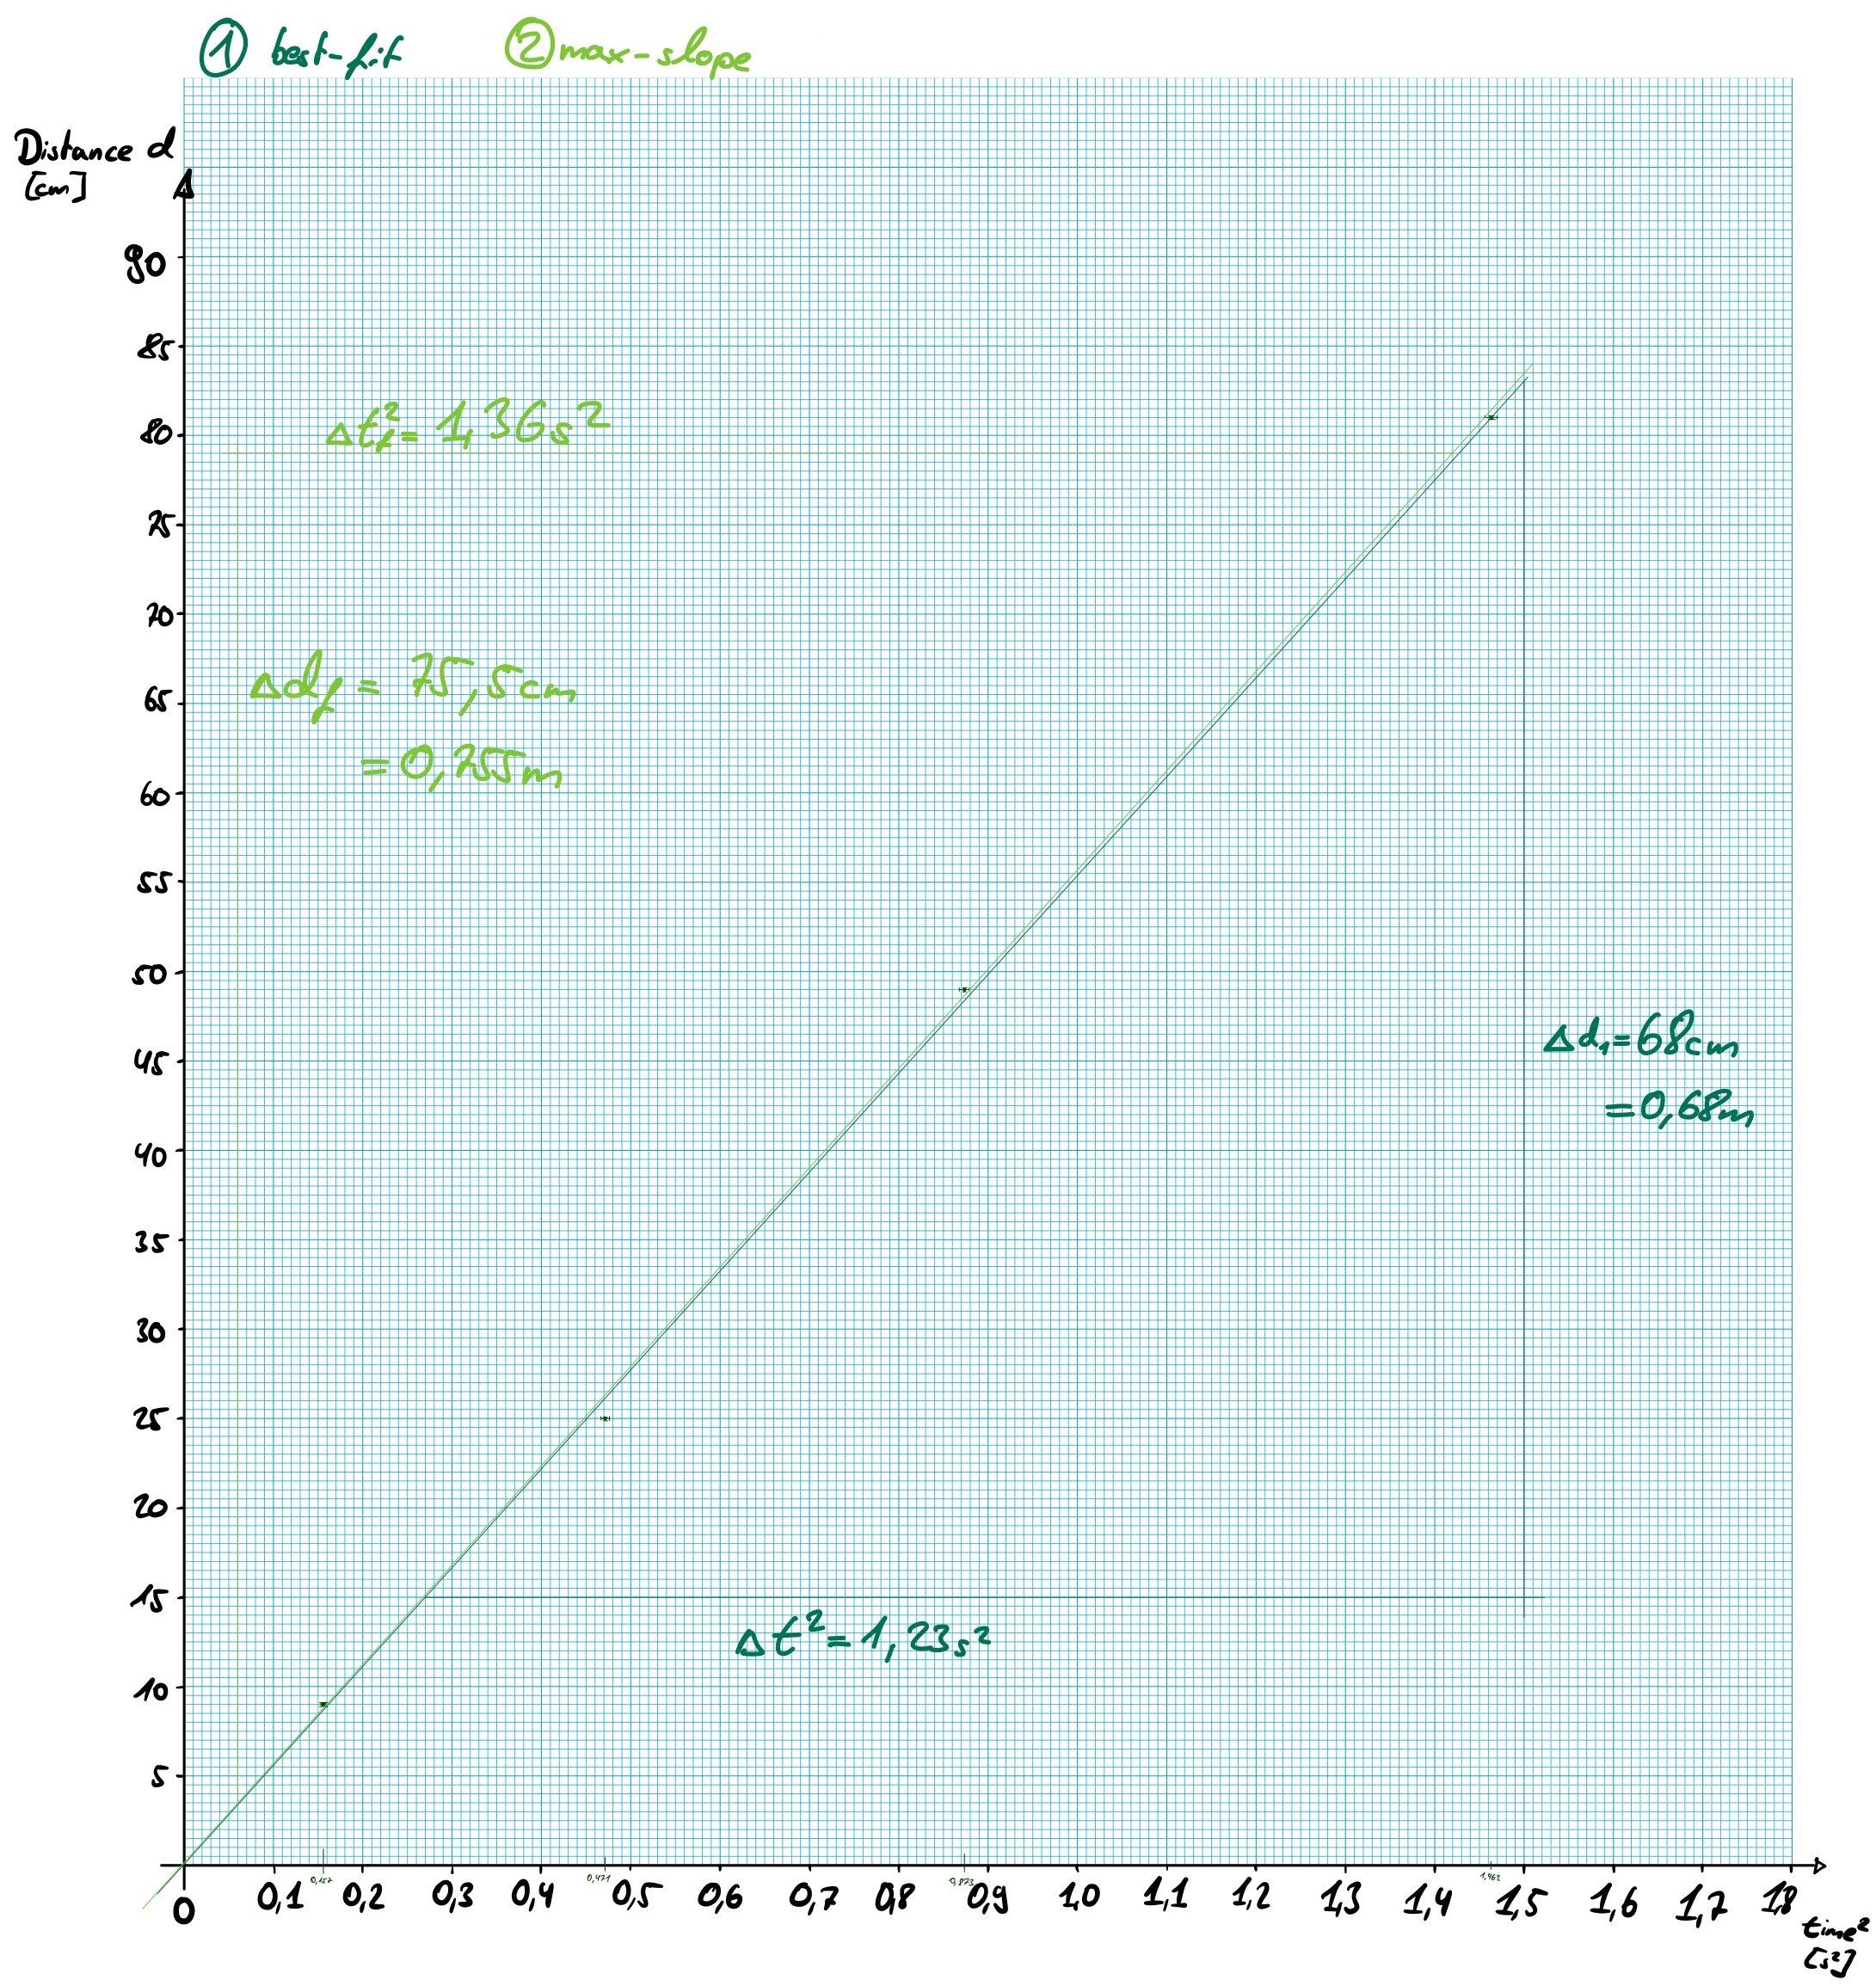
\includegraphics[width=20cm, angle=90]{graphics/dia1.pdf}}
\end{figure}


\newpage

\subsection{Calibration of the Pt100 thermometer}

We begin by evaluating the temperature values of the gas thermometer's pressure measurements from 0$^{\circ}$C to 100$^{\circ}$C from table 2 using the previously drawn graph and applying the same method as before. The used diagram is shown in figure 5 and the results are presented in table 6.

\begin{table}[!ht]
    \centering
    \begin{tabular}{c|c}
    $\bm{p}$ [hPa] & $\bm{T}$ [$^{\circ}$C] \\ \hline
    $966 \pm 1$  & $16 \pm 1$ \\
    $997 \pm 1$  & $23 \pm 1$ \\
    $1030 \pm 1$  & $33 \pm 1$ \\
    $1066 \pm 1$  & $44 \pm 1$ \\
    $1099 \pm 1$  & $53 \pm 1$ \\
    $1139 \pm 1$  & $65 \pm 1$ \\
    $1174 \pm 1$  & $75 \pm 1$ \\
    $1209 \pm 1$  & $85 \pm 1$ \\
    $1240 \pm 1$  & $95 \pm 1$ \\
    \end{tabular}
    \caption{temperature values from the gas thermometer}
\end{table}

We want to create another diagram with the resistance of the Pt100 thermometer against the evaluated temperatures of the gas thermometer in the range from 0$^{\circ}$C to 100$^{\circ}$C. First, we calculate the resistance $R$ for each measured voltage $U$ from table 2 using $R=\frac{U}{I}$, $I$ being the current provided by the 1mA source. But since the current is 1mA and the Voltage is given in mV, the values of the voltage and resistance are the same. Therefore we get the simple following relations shown in table 7.
%Then, using equation \textbf{XXX} with the given values for $A$ and $B$, we calculate the according temperatures and with equation \textbf{XXX} their error.


\begin{table}[!ht]
    \centering
    \begin{tabular}{c|c|c}
    $\bm{U}$ [mV] & $\bm{R}$ [$\Omega$] & $\bm{T}$ [$^{\circ}$C] \\ \hline
    $101,5 \pm 1,6$  & $101,5 \pm 1,6$  & $0$ \\
    $105,9 \pm 1,6$  & $105,9 \pm 1,6$  & $16 \pm 1$ \\
    $109,2 \pm 1,6$  & $109,2 \pm 1,6$  & $23 \pm 1$ \\
    $113,2 \pm 1,6$  & $113,2 \pm 1,6$  & $33 \pm 1$ \\
    $117,1 \pm 1,6$  & $117,1 \pm 1,6$  & $44 \pm 1$ \\
    $120,8 \pm 1,6$  & $120,8 \pm 1,6$  & $53 \pm 1$ \\
    $125,5 \pm 1,6$  & $125,5 \pm 1,6$  & $65 \pm 1$ \\
    $129,4 \pm 1,6$  & $129,4 \pm 1,6$  & $75 \pm 1$ \\
    $133,7 \pm 1,6$  & $133,7 \pm 1,6$  & $85 \pm 1$ \\
    $137,1 \pm 1,6$  & $137,1 \pm 1,6$  & $95 \pm 1$ \\
    $139,4 \pm 1,6$  & $139,4 \pm 1,6$  & $100$
    \end{tabular}
    \caption{resistance and temperature for the Pt100}
\end{table}

Now we create the diagram shown in figure 6 using the values from the table above and assigning the temperature $T$ to the x-axis and the resistance $R$ to the y-axis. We insert a best-fit and a max-slope line and estimate their slopes $m_1$ and $m_2$ respectively as well as the error $\Delta m_1$:

\begin{equation}
    \begin{split}
        m_1 &= \frac{\Delta R_1}{\Delta T_1} = 0,393 \frac{\Omega}{^{\circ}\text{C}} \\
        m_2 &= \frac{\Delta R_2}{\Delta T_2} = 0,411 \frac{\Omega}{^{\circ}\text{C}} \\
        \Delta m_1 &= | m_1 - m_2 | = 0,019 \frac{\Omega}{^{\circ}\text{C}} \\ \\
        \implies \bm{m_1} &= \bm{(0,393 \pm 0,019) \frac{\Omega}{^{\circ}\textbf{C}}}
    \end{split}
\end{equation}

To compare the estimated value for $m_1$, we can calculate the slope $m_p$ of the linear term of the polynomial from equation 2 using the given values for $A$ and $R_0$:

\begin{equation}
    \begin{split}
        R(T) &= R_0 (1+AT) \\ \\ 
        \implies m_p &= R_0 A = 0,391 \frac{\Omega}{^{\circ}\text{C}}
    \end{split}
\end{equation}

If we compare the values of $m_1$ and $m_p$ we get:

\begin{equation}
    \sigma = \frac{\left| m_1 - m_p \right|}{\Delta m_1} = 0,11
\end{equation}

Which is an insignificant difference.

\begin{figure} [!p]
    \centering
    \caption{determining the measurements of the gas thermometer}
    \makebox[\textwidth][c]{
    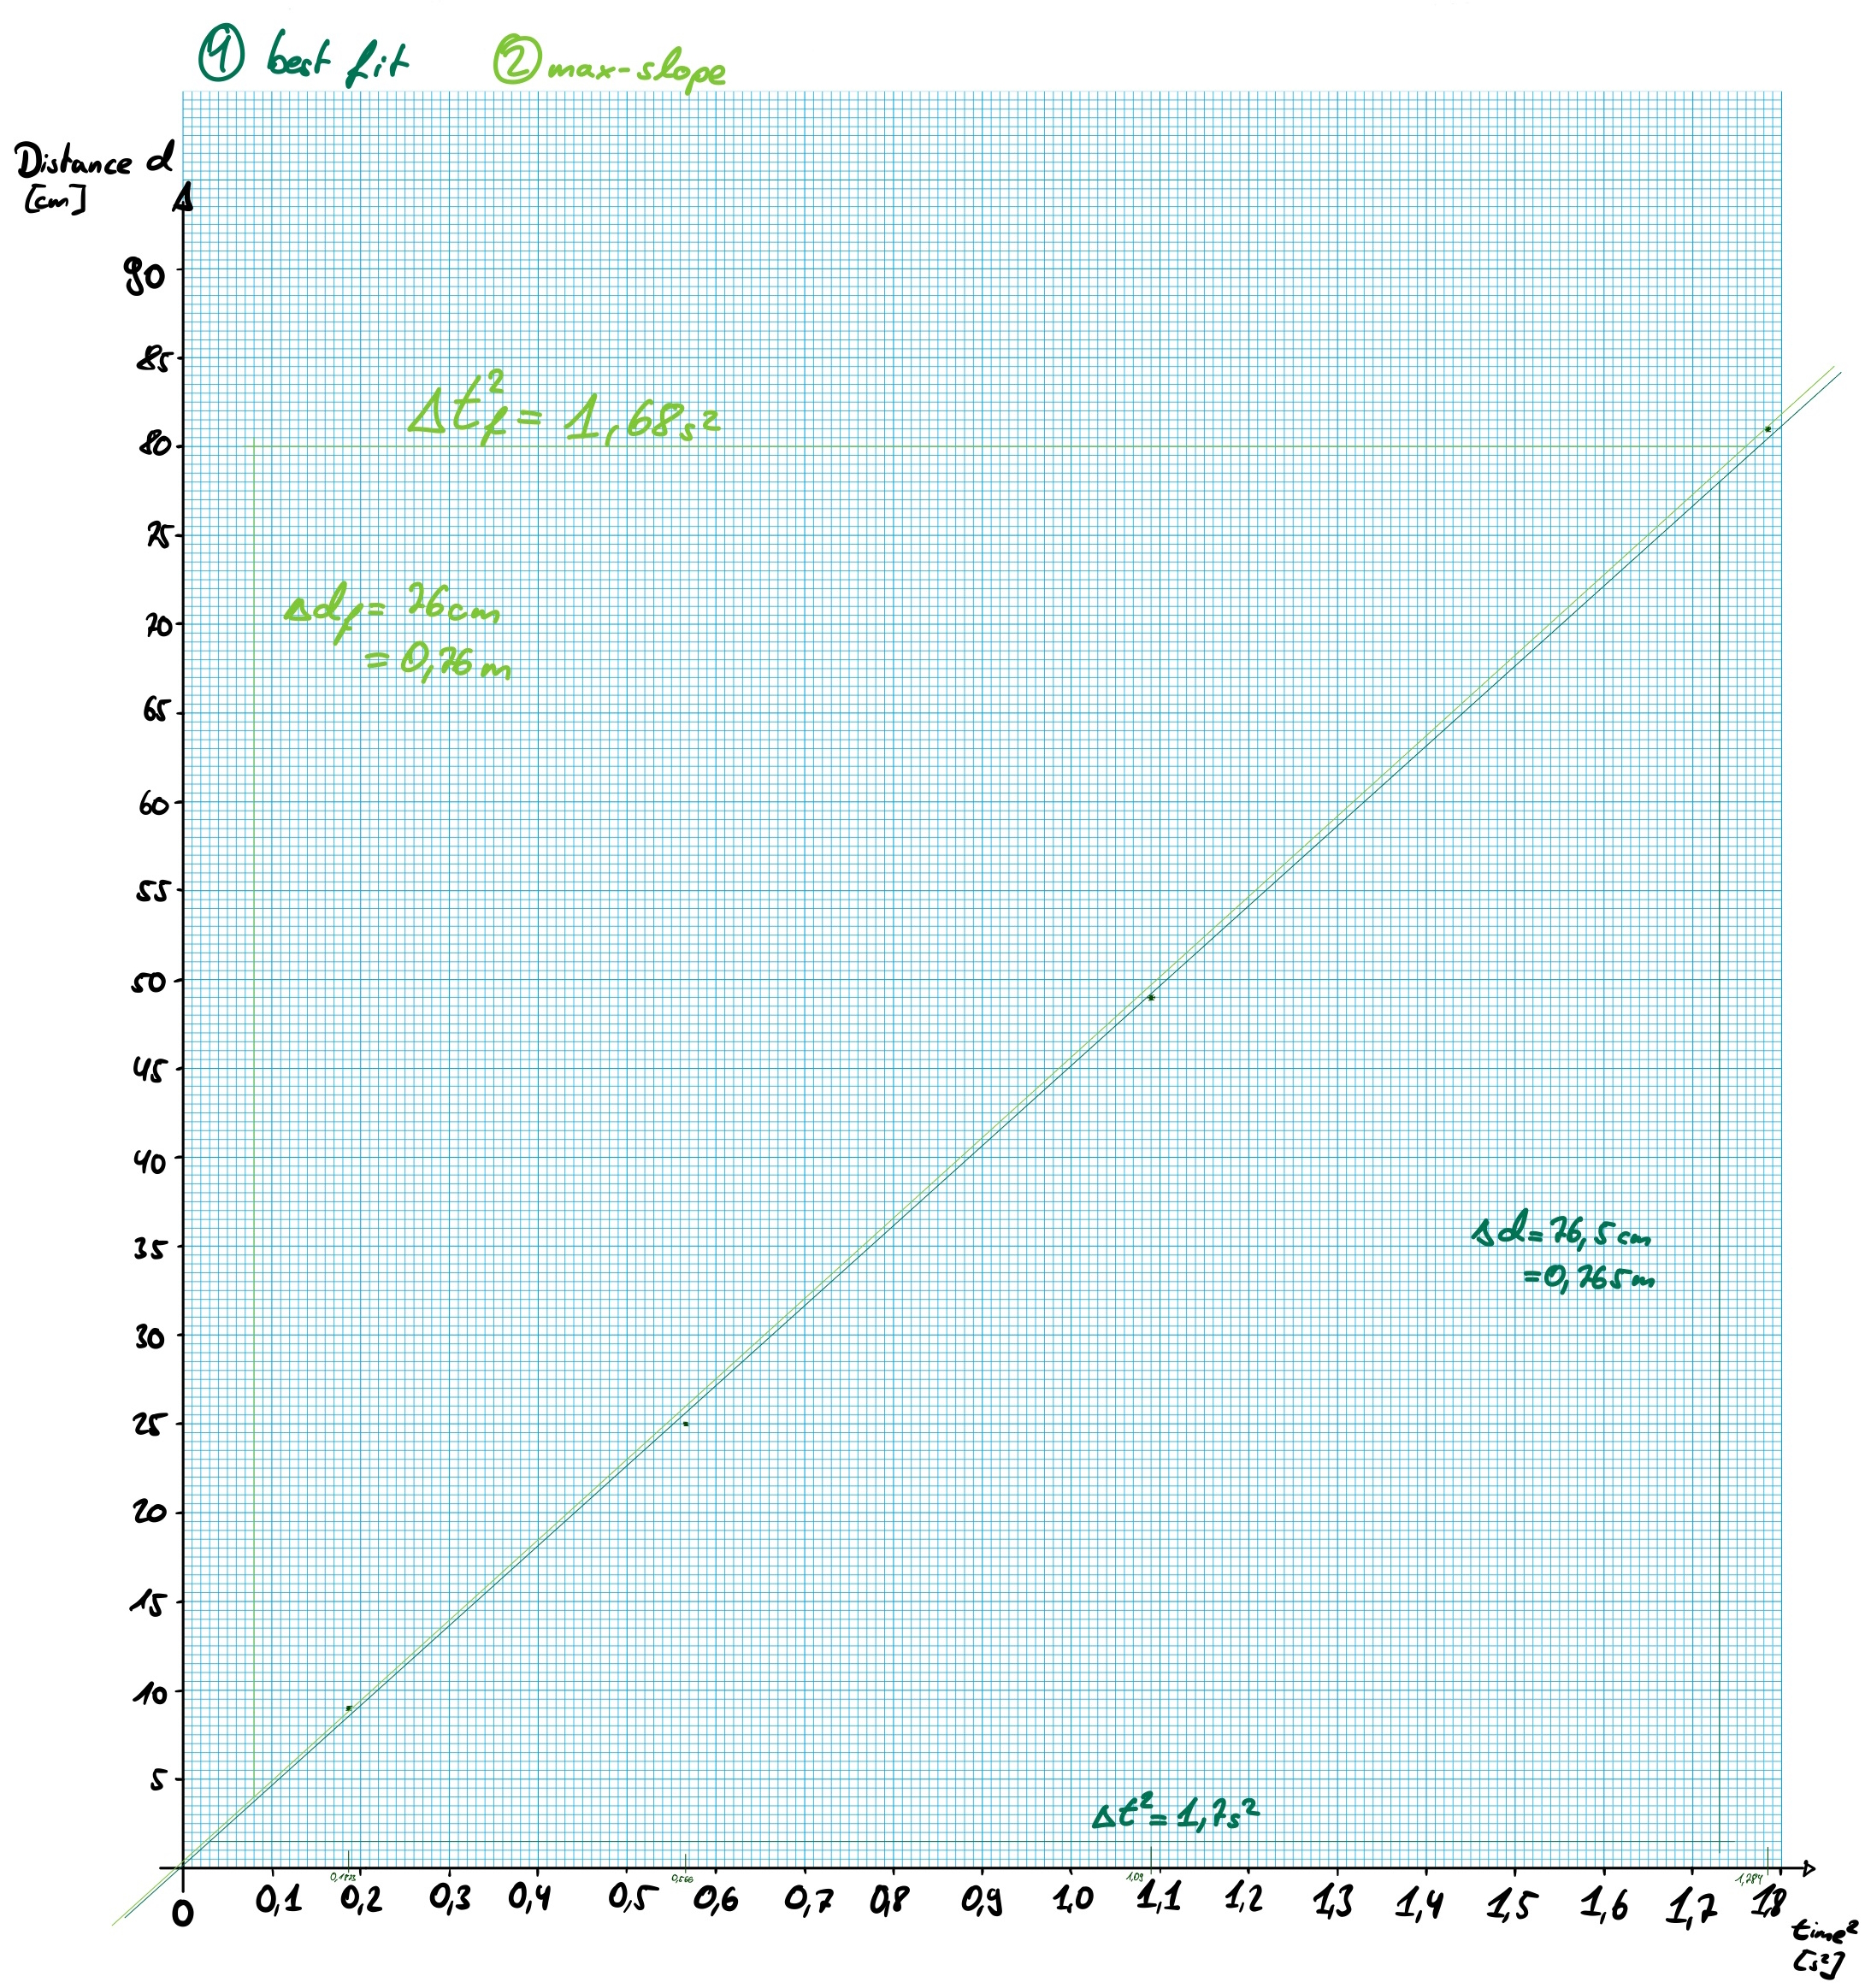
\includegraphics[width=20cm, angle=90]{graphics/dia2.pdf}}
\end{figure}

\begin{figure} [!p]
    \centering
    \caption{Pt100: resistance against temperatures}
    \makebox[\textwidth][c]{
    \includegraphics[width=20cm, angle=90]{graphics/dia3.pdf}}
\end{figure}

\newpage

\subsection{Temperature measurements of the pyrometer and gas thermometer}

To compare the measurements of the pyrometer and the gas thermometer, the measured temperatures are applied against each other in a diagram, shown in figure 7. We insert the values depicted in table 8, taken from table 4 and the previous calculations. 

\begin{table}[!ht]
    \centering
    \begin{tabular}{c|c}
    $\bm{T_{gt}}$ [$^{\circ}$C] & $\bm{T_{p}}$ [$^{\circ}$C] \\ \hline
    $0$ & $-1,3 \pm 2,0$  \\
    $16 \pm 1$ & $10,9 \pm 2,2$  \\
    $23 \pm 1$ & $20,3 \pm 2,3$  \\
    $33 \pm 1$ & $30,0 \pm 2,5$  \\
    $44 \pm 1$ & $40,2 \pm 2,6$  \\
    $53 \pm 1$ & $49,8 \pm 2,7$  \\
    $65 \pm 1$ & $59,9 \pm 2,9$  \\
    $75 \pm 1$ & $70,1 \pm 3,1$  \\
    $85 \pm 1$ & $80,0 \pm 3,2$  \\
    $95 \pm 1$ & $89,2 \pm 3,3$  \\
    $100$ & $93,6 \pm 3,4$ 
    \end{tabular}
    \caption{temperature measurements: gas thermometer $T_{gt}$ \& pyrometer $T_{p}$}
\end{table}

Again, we calculate the slope of the best-fit line $m_t$ and it's error the same way as before:

\begin{equation}
    \begin{split}
        m_t &= \frac{\Delta T_{p_1}}{\Delta T_{gt_1}} = 0,97 \\
        \Delta m_t &= \left| m_t - \frac{\Delta T_{p_2}}{\Delta T_{gt_2}} \right| = 0,04\\ \\
        \implies \bm{m_t} &= \bm{0,97 \pm 0,04} 
    \end{split}
\end{equation}

Now theoretically, this slope should be equal to 1 since we would expect to measure the same temperature with both devices. But as we can see, this is not quite the case. Comparing our calculated slope $m_t$ to the ideal value of 1 gives a difference of $\sigma = 0,075$, which is an insignificant difference.

\begin{figure} [!p]
    \centering
    \caption{comparing the gas thermometer and pyrometer}
    \makebox[\textwidth][c]{
    \includegraphics[width=\textwidth]{graphics/dia4.pdf}}
\end{figure}

\newpage

\subsection{Temperature of the flames}

Finally, we want to analyze the measured thermoelectric voltages given by the thermocouple when recording the two flames, one with high and one with low air supply. The according temperatures are taken from the calibration table matching the used device. On that note it is important to mention that all these temperature values are only educated guesses based on the approximate location of the measured voltages on the table as well as the approximate error intervals. More precise values would need far more accurate tables as the ones given, which gave temperature values in intervals of 10$^{\circ}$C. The results are shown in table 9 and figure 8 shows the according points in the flame.

\begin{table}[!ht]
    \centering
    \begin{tabular}{c|c|c}
        \textbf{flame} & \textbf{$\bm{U}$} [mV] & $T$ [°C] \\ \hline
        low air supply & $3,4 \pm 1,5$ & $410 \pm 150$ \\ 
        ~ & $6,2 \pm 1,5$ & $690 \pm 140$ \\ 
        ~ & $7,2 \pm 1,5$ & $790 \pm 150$ \\ 
        ~ & $4,7 \pm 1,5$ & $550 \pm 150$ \\ 
        ~ & $3,5 \pm 1,5$ & $430 \pm 150$ \\ \hline
        high air supply & $6,5 \pm 1,5$ & $720 \pm 140$ \\ 
        ~ & $7,8 \pm 1,5$ & $840 \pm 140$ \\ 
        ~ & $9,5 \pm 1,5$ & $990 \pm 130$ \\ 
        ~ & $11 \pm 1,5$ & $1120 \pm 130$ \\ 
        ~ & $11,6 \pm 1,5$ & $1170 \pm 130$ \\ 
    \end{tabular}
    \caption{calculated errors of part 3}
\end{table}

\begin{figure} [!h]
    \centering
    \includegraphics[width=10cm]{graphics/sketchflame.jpg}
    \caption{temperatures of different parts of the flames}
\end{figure}

\newpage
%---------------PRÄSENTATION DER ENDERGEBNISSE---------------
\section{Presentation of final results}

This experiment saw three different methods of measuring temperature using three different devices. 

Firstly, we used measurements from the gas thermometer to calculate the temperature of the point, where all pressure is zero $T_0$, the temperature of liquid nitrogen $T_N$, and the temperature of dry ice $T_{DI}$:

\begin{equation}
    \begin{split}
        \bm{T_0} &= \bm{-(268 \pm 4)^{\circ}} \textbf{C} \\
        \bm{T_N} &= \bm{-(195 \pm 1)^{\circ}\textbf{C}} \\
        \bm{T_{DI}} &= \bm{-(45 \pm 1)^{\circ}\textbf{C}}
    \end{split}
\end{equation}

Then, using the measurements from the Pt100 resistance thermometer, we calculated the slope of the best-fit graph when plotting the measured resistance against the temperature:

\begin{equation}
\bm{m_1} = \bm{(0,393 \pm 0,019) \frac{\Omega}{^{\circ}\textbf{C}}}
\end{equation}

Afterwards, we compared the measurements of the gas thermometer and pyrometer by plotting the measured temperatures against each other and again determining the slope of the best-fit graph:

\begin{equation}
    \begin{split}
    \bm{m_t} = \bm{0,97 \pm 0,04} 
    \end{split}
\end{equation}

Finally, we evaluated the measurements of the thermocouple of the two flames to determine the different temperatures in different parts of the flames:

\begin{figure} [!h]
    \centering
    \includegraphics[width=7cm]{graphics/sketchflame.jpg}
\end{figure}

\newpage
%---------------ZUSAMMENFASSUNG UND DISKUSSION---------------
\section{Summary and Discussion}

In this experiment we recorded different temperatures using different thermometers ranging from liquid nitrogen at -195$^{\circ}$C up to the flame of a Bunsen burner at 1170$^{\circ}$C.

The first notable thing regarding this experiment would be, that all measurements, observations, and results were within our expectations as well as the margins of errors. All results made sense when compared to literature or ideal vales. Parts 1 and 2 always showed great results in comparison with ideal values, but especially part 3 with it's deviation of $\sigma = 0,075$ when comparing our measured slope to the ideal calculated value showed a surprisingly accurate result. Part 4 also delivered values that resembled the expected characteristics of a flame, where for the low air supply flame the temperature rises further from the flame up to a certain point to then drop off and for the high air supply one to burn hottest close to the source and gradually decrease going upwards.

Nevertheless, there are still points to be noted, where improvements could further improve the results.

Firstly, during the experiment there were some challenging aspects, one being heating up the liquid in somewhat accurate increments of 10$^{\circ}$C, which turned out to be quite far off in our measurements all the time. Additionally, when we comparing the measurements of the gas thermometer and pyrometer, we noticed that the pyrometer always seemed to record slightly lower temperatures in comparison, which could be due to the different points the measurements were taken. The glass ball of the gas thermometer was completely submerged in the liquid, whilst the pyrometer was always aimed at the surface. This directly leads to the second noticeable room for improvement, which is the even heat distribution inside the liquid. Even though a magnetic stirrer was used to mix the liquid, the results from comparing the measurements of the gas thermometer and pyrometer suggest that the surface still had a slightly lower temperature than the lower parts inside the liquid. 

Moving on, in the final part of this experiment, recording the different parts of the flames turned out to be quite challenging. Since the windows needed to be open when using the Bunsen burner regarding safety reasons, the flame was in constant motion and it was hard to focus the thermocouple at one specific point. Also, the room temperature was noticeably shifting during our time experimenting, which also impacts the accuracy of the absolute temperature value calculated from the thermocouple measurements.

Generally, we also need to mention the predetermined inaccuracy of calculating results graphically per hand. Manually inserting points, finding best-fit as well as maximum-slope lines, and reading values off of diagrams is always faulty to some degree. The assistance of computer programs would have definitely given more accurate results. 

To conclude, despite the mentioned potential errors, all results taken from this experiment showed no deviation from expected outcomes and were well within the 3$\sigma$-intervals when compared to literature values.

\end{document}

